\section{Методика использования программного средства}
\label{sec:manual}

В данном разделе приведены основные сведения по работе с программным средством. 

Приложения данного дипломного проекта (а точнее, его клиентская часть) не требует настройки на конечных устройствах пользователя. Достаточно лишь
полной установки, так как оно представляет из себя настольное приложение. Как и было заявлено в требованиях, для корректной работы программного средства
требуется операционная система Windows 10, а также пакет следующих системных библиотек:
\begin{itemize}
	\item .NET Framework 4.8;
	\item Visual C++ Redistributable.
\end{itemize} 

Далее расмотренны основные функции, предоставляемые приложениями.

Приложение-тестер необходимо для создания новых и редактирования существующих пакетов вопросов. Интерфейс приложения имеет следующий вид (рисунок \ref{sec:manual:tester}): 

\begin{figure}[!ht]
    \centering
    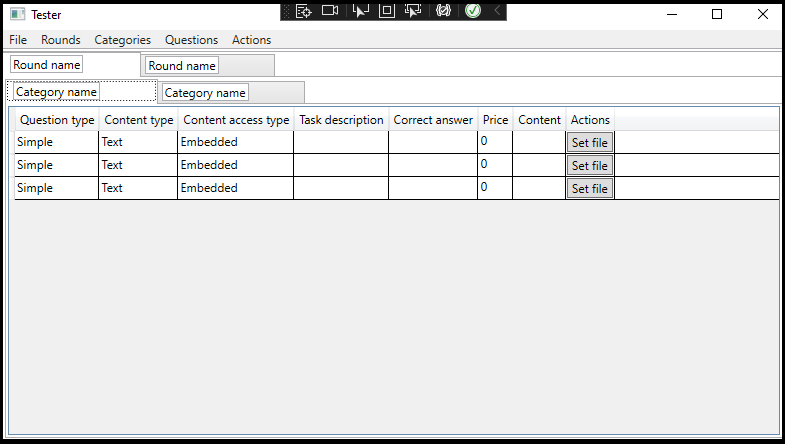
\includegraphics[scale=0.75]{attachments/tester.png}
    \caption{Интерфейс приложения-тестера}
    \label{sec:manual:tester}
\end{figure}

Для того, чтобы создать новый пакет вопросов необходимо использовать сочетание клавиш CTRL+N,F либо их аналог на панели меню. Для открытия уже существующего пакета можно 
воспользоваться сочетанием CTRL+O. Для сохранения созданного или редактированного пакета можно воспользоваться сочетанием CTRL+S.

Для того, чтобы добавить новый раунд в викторину можно воспользоваться сочетанием клавиш CTRL+N,R. Список раундов отображается сверху, каждый раунд обладает своим именем. Рекомендуется давать осмысленные
имена, хотя ограничений на это нет. Для удаления уже добавленного раунда можно воспользоваться сочетанием CTRL+D,R. Следует отметить, что вместе с раундом будут удалены все категории, связанные с ним.

Для добавления новой категории в раунд можно воспользоваться сочетанием клавиш CTRL+N,C. Аналогично с раундами каждая категория имеет свое имя,
рекомендуется называть категории в соответствии с тематикой вопросов, находящихся в ней. Для удаления категории можно воспользоваться сочетанием CTRL+D,C. Следует отметить,
что вместе с категорией будут удалены все вопросы, относящиеся к удаляемой категории, поэтому следует соблюдать осторожность. 

Для добавления нового вопроса можно использовать сочетание клавиш CTRL+N,Q, а для удаления CTRL+D,R соответственно. Редактирование вопросов происходит непосредственно
в результате редактирования соотвествующей строки в таблице.

При сохранении пакета запускаются валидации введенных данных, в случае возникновения ошибок информацию можно получить в соответствующем окне (рисунок \ref{sec:manual:tester_err}).
Все пакеты с вопросами сохраняются на диск в формате .qpck. В дальнейшем эти файлы можно использовать в клиенте при создании викторин.

\begin{figure}[!ht]
    \centering
    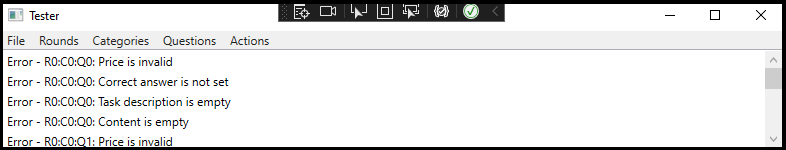
\includegraphics[scale=0.75]{attachments/tester_err.png}
    \caption{Пример валидационных ошибок тестера}
    \label{sec:manual:tester_err}
\end{figure}

Приложение-клиент является основным для использования и служит для непосредственно проведения многопользовательских викторин. 
Экран авторизации выглядит следующим образом (рисунок \ref{sec:manual:identity_ui}).

\begin{figure}[!ht]
    \centering
    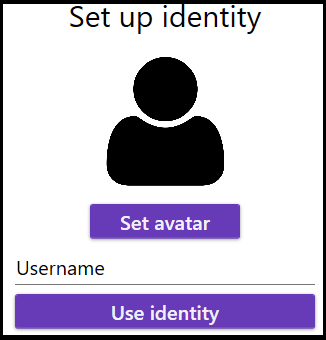
\includegraphics[scale=1]{attachments/identity_ui.png}
    \caption{Окно авторизации}
    \label{sec:manual:identity_ui}
\end{figure}

Здесь можно задать идентичность, по которой знакомые смогут опознать игрока. Из настраиваемых параметров имя пользователя и аватар, при этом если пользователь по какой-либо
причине не имеет желания устанавливать в качестве аватара собственное изображение, то будет использоваться изображение по умолчанию.

Главное меню (рисунок \ref{sec:manual:menu_ui}) служит для навигации между другими окнами. Здесь пользователь может создать новое лобби, присоединится к существующему, поменять авторизационные данные, а
также выйти из приложения.

\begin{figure}[!ht]
    \centering
    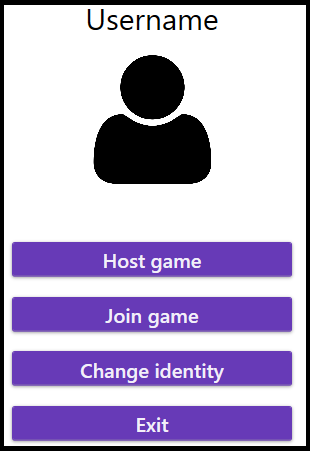
\includegraphics[scale=0.8]{attachments/menu_ui.png}
    \caption{Главное меню приложения}
    \label{sec:manual:menu_ui}
\end{figure}

На экране создания лобби (рисунок \ref{sec:manual:host_ui}) пользователь может стать организатором собственной викторины. Для этого достаточно выбрать набор вопросов из 
уже существующих, либо заранее создать его самостоятельно, а также задать имя лобби и, по желанию, пароль. Если пользователь попал сюда по ошибке то можно вернуться в меню с
помощью кнопки <<Back to menu>>.

\begin{figure}[!ht]
    \centering
    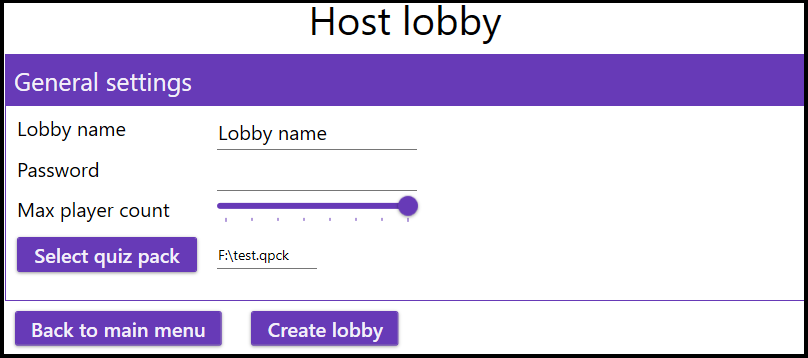
\includegraphics[scale=0.7]{attachments/host_ui.png}
    \caption{Окно создания лобби}
    \label{sec:manual:host_ui}
\end{figure}

На экране присоединения к лобби (рисунок \ref{sec:manual:join_ui}) пользователь может присоединиться к уже созданным кем-то лобби. Для этого достаточно выбрать лобби из списка 
и нажать <<Join>>/ если в лобби есть пароль, то его необходимо правильно ввести.

\begin{figure}[!ht]
    \centering
    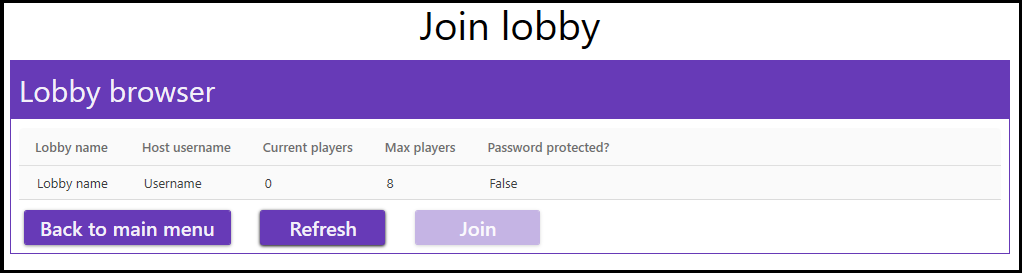
\includegraphics[scale=0.6]{attachments/join_ui.png}
    \caption{Окно присоединения к лобби}
    \label{sec:manual:join_ui}
\end{figure}

На экране игрового лобби (рисунок \ref{sec:manual:lobby_ui}) непосредственно просходит игровой процесс. Сюда можно попасть в качестве организатора создав лобби либо в качестве игрока присоединившись к нему.

\begin{sidewaysfigure}
\centering
    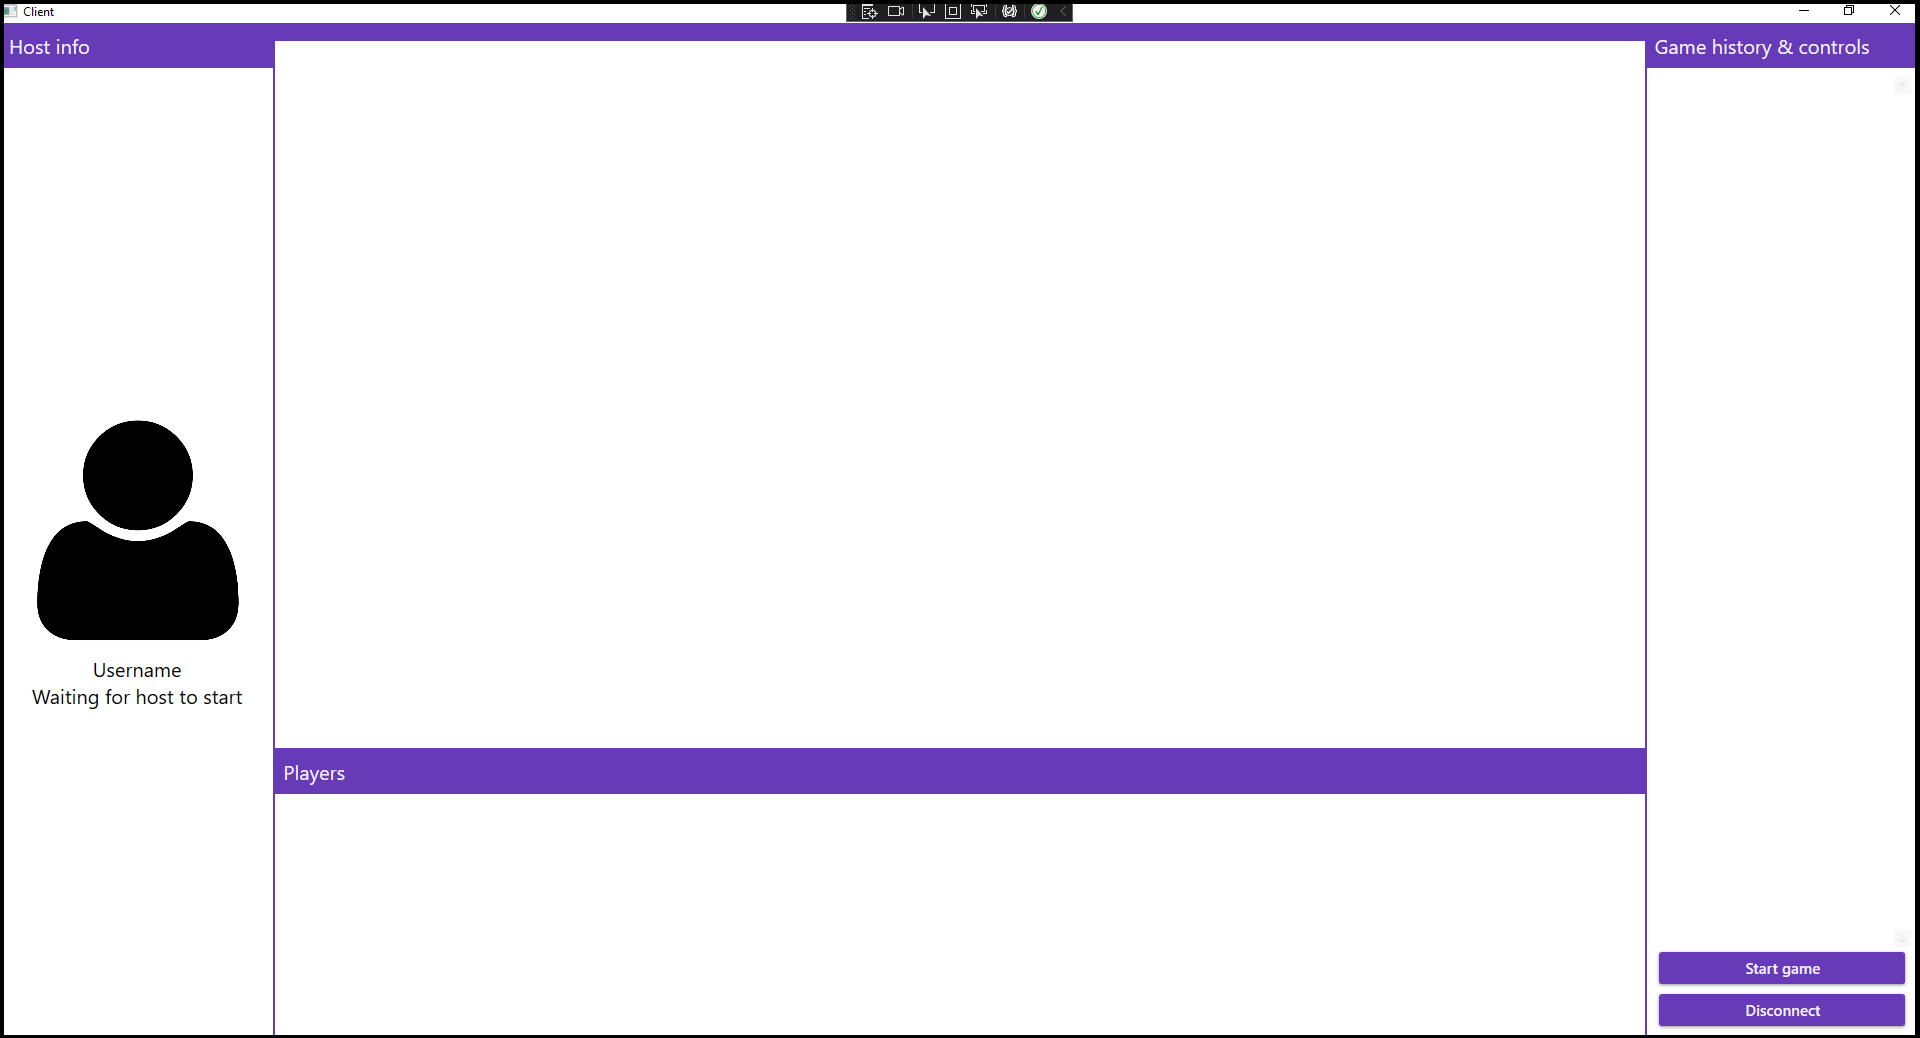
\includegraphics[scale=0.45]{attachments/lobby_ui.png}
    \caption{Окно игрового лобби}
    \label{sec:manual:lobby_ui}
\end{sidewaysfigure}

Организатор следит за игровым процессом и контролирует правильность ответов. Игроки отвечают на вопросы и зарабатывают очки. Победитель определяется по исчерпанию всех вопросов
на основе наибольшего количества очков.